\documentclass[a4paper]{article}

\usepackage[T1]{fontenc}
\usepackage[utf8x]{inputenc}

\usepackage[a4paper]{geometry}
\geometry{verbose,tmargin=3cm,bmargin=3cm,lmargin=2cm,rmargin=2cm,headheight=2cm,headsep=1cm,footskip=2cm}

\usepackage{fancyhdr}
\pagestyle{fancy}
\setlength{\parskip}{\medskipamount}
\setlength{\parindent}{0pt}
\usepackage{graphicx}

\makeatletter

\usepackage{float} 
\usepackage{lastpage}
\usepackage{indentfirst}

\usepackage{pgf}
\usepackage{tikz}
\usetikzlibrary{arrows,automata, shapes, positioning, calc}

\lhead[lh-even]{Edgar Vedvik (edgarmv)\\ Informatikk (BIT)}
\chead[ch-even]{TDT4205 Kompilatorteknikk\\ Problem Set 4 }
\rhead[rh-even]{\today}

\lfoot[lf-even]{}
\cfoot[cf-even]{Side \thepage{} av \pageref{LastPage}}
\rfoot[rf-even]{}

\date{}

\makeatother

\usepackage[english]{babel}

\begin{document}


\thispagestyle{fancy}

\section{Theory}
\subsection{}

There are shift/reduce conflicts in $I_{10}$ and $I_{12}$ since we don't know if whe should reduce \textbf{a}B to A and EB to D or look for \textbf{b} and shift it. This is because we have no lookahead. If we had a LR(1) automaton the shift/reduce conflicts would be resolved.

\begin{figure*}[h]
    \centering
    \scalebox{.9}{
    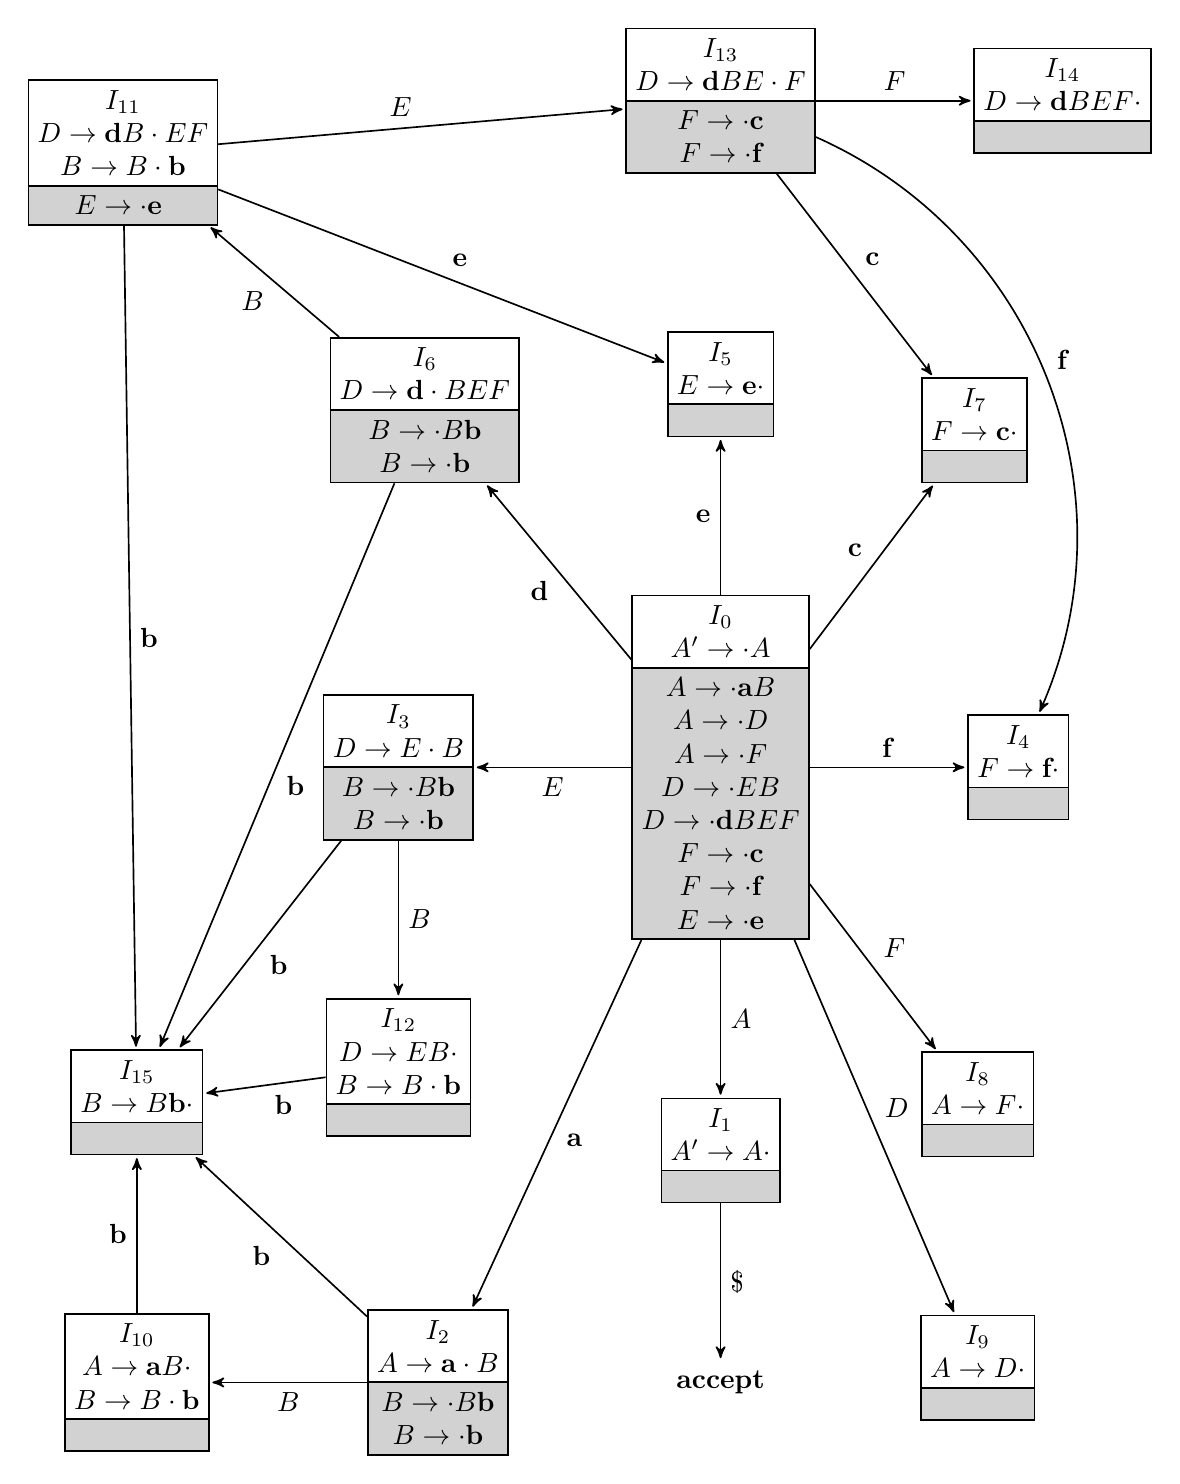
\begin{tikzpicture}
        [->, >=stealth', shorten >=1pt, auto, node distance=2cm, semithick,
        itemset/.style={rectangle split, rectangle split parts=2, rectangle split part fill={white, lightgray!70}, align=center, draw=black}]
        \node[itemset]  (I0)
        {$I_0$ \\
            $A' \rightarrow \cdot A$
            \nodepart{two}
            $ A  \rightarrow \cdot \textbf{a}  B $ \\
            $ A  \rightarrow \cdot D$ \\
            $ A  \rightarrow \cdot F$ \\
            $ D  \rightarrow \cdot EB$ \\
            $ D  \rightarrow \cdot \textbf{d} BEF$ \\
            $ F  \rightarrow \cdot \textbf{c}$ \\
            $ F  \rightarrow \cdot \textbf{f}$ \\
            $ E  \rightarrow \cdot \textbf{e}$
        };

        \node[itemset]  (I1)    [below = of I0]
        {$I_1$ \\
            $ A'  \rightarrow  A  \cdot$
        };
        
        \node[draw=none, fill=none]  (accept)    [below = of I1] {\textbf{accept}};

        \node[itemset]  (I2)    [left = of accept]
        {$I_2$ \\
            $ A  \rightarrow  \textbf{a} \cdot B$
            \nodepart{two}
            $ B \rightarrow \cdot B \textbf{b} $\\
            $ B \rightarrow \cdot \textbf{b} $
        };

        \node[itemset]  (I3)    [left = of I0]
        {$I_3$ \\
            $ D  \rightarrow E \cdot B$
            \nodepart{two}
            $ B \rightarrow \cdot B \textbf{b}$ \\
            $ B \rightarrow \cdot \textbf{b}$
        };

        \node[itemset]  (I8)    [below right = of I0]
        {$I_8$ \\
            $ A  \rightarrow  F \cdot$
        };

        \node[itemset]  (I5)    [above = of I0]
        {$I_5$ \\
            $ E  \rightarrow \textbf{e} \cdot$
        };

        \node[itemset]  (I6)    [above left = of I0]
        {$I_6$ \\
            $ D  \rightarrow \textbf{d} \cdot BEF$
            \nodepart{two}
            $ B \rightarrow \cdot B \textbf{b}$ \\
            $ B \rightarrow \cdot \textbf{b}$
        };

        \node[itemset]  (I7)    [above right = of I0]
        {$I_7$ \\
            $ F  \rightarrow \textbf{c} \cdot$
        };

        \node[itemset]  (I4)    [right = of I0]
        {$I_4$ \\
            $ F  \rightarrow \textbf{f} \cdot$
        };

        \node[itemset]  (I9)    [below = of I8]
        {$I_9$ \\
            $ A  \rightarrow  D \cdot$
        };

        \node[itemset]  (I10)    [left = of I2]
        {$I_{10}$ \\
            $ A  \rightarrow \textbf{a} B \cdot$ \\
            $ B  \rightarrow B \cdot \textbf{b} $
        };
        
        \node[itemset]  (I11)    [above left = of I6]
        {$I_{11}$ \\
            $ D  \rightarrow \textbf{d} B \cdot EF$ \\
            $ B  \rightarrow B \cdot \textbf{b} $
            \nodepart{two}
            $ E \rightarrow \cdot \textbf{e} $
        };

        \node[itemset]  (I12)    [below = of I3]
        {$I_{12}$ \\
            $ D  \rightarrow EB \cdot$ \\
            $ B  \rightarrow B \cdot \textbf{b} $
        };

        \node[itemset]  (I13)    [above = of I5]
        {$I_{13}$ \\
            $ D  \rightarrow \textbf{d} BE \cdot F$
            \nodepart{two}
            $ F \rightarrow \cdot \textbf{c}$ \\
            $ F \rightarrow \cdot \textbf{f}$
        };

        \node[itemset]  (I14)    [right = of I13]
        {$I_{14}$ \\
            $ D  \rightarrow \textbf{d} BEF \cdot$
        };
        
        \node[itemset]  (I15)    [above = of I10]
        {$I_{15}$ \\
            $ B  \rightarrow B \textbf{b} \cdot$
        };

        \path (I0) edge                 node {$ A $}                    (I1)
              (I0) edge                 node {\textbf{a}}               (I2)
              (I0) edge                 node {\textbf{e}}               (I5)
              (I0) edge                 node {\textbf{f}}               (I4)
              (I0) edge                 node {$E$}                      (I3)
              (I0) edge                 node {\textbf{d}}               (I6)
              (I0) edge                 node {\textbf{c}}               (I7)
              (I0) edge                 node {$F$}                      (I8)
              (I0) edge                 node {$D$}                      (I9)
              (I1) edge                 node {\$}                       (accept)
              (I2) edge                 node {$B$}                      (I10)
              (I2) edge                 node {\textbf{b}}               (I15)
              (I3) edge                 node {$B$}                      (I12)
              (I3) edge                 node {\textbf{b}}               (I15)
              (I6) edge                 node {$B$}                      (I11)
              (I6) edge                 node {\textbf{b}}               (I15)
              (I10) edge                node {\textbf{b}}               (I15)
              (I11) edge                node {$E$}                      (I13)
              (I11) edge                node {\textbf{b}}               (I15)
              (I11) edge                node {\textbf{e}}               (I5)
              (I12) edge                node {\textbf{b}}               (I15)
              (I13) edge                node {$F$}                      (I14)
              (I13) edge  [bend left=45]   node {\textbf{f}}               (I4)
              (I13) edge                node {\textbf{c}}               (I7);
      \end{tikzpicture}}
    \caption{The LR(0) automaton} \label{fig:prob2aautomaton}
\end{figure*}

\subsection{SLR}

The grammar is not SLR(1). It is ambigious in state $I_{10}$ and $I_{12}$. Because it has a shift/reduce conflict.

\end{document}
